
\chapter{Results and Discussion}

The simulator capture sets of five perspective images and converts them into one image, mimicking the effect of fisheye lenses cameras. Using the setup described in Section~\ref{sec:combining_pictures}, and an calibratable polynomial lens model, each images is mapped onto specific parts of the final fisheye image. In Figure~\ref{fig:res_show_fisheye} the complete image is shown, simulating a $270^\circ$ FoV camera mounted beneath the multirotor during flight. The simulator is fully implemented for Linux, but will work on Windows with some modifications to the build system and client program. This includes removing the ROS publisher, as ROS is currently not available on Windows platforms. No part of the simulator has been tested on Mac OS. 

\begin{figure}[!htb]
    \centering
    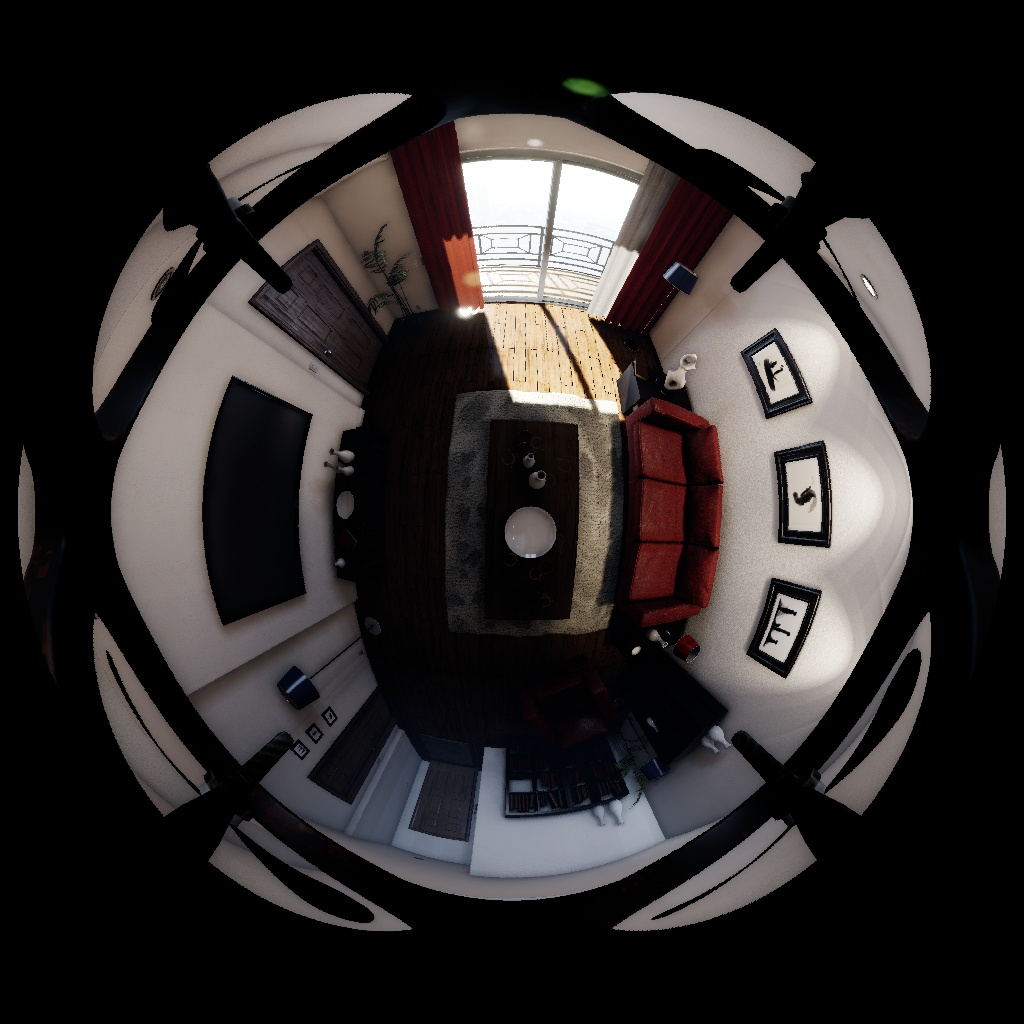
\includegraphics[width=0.7\textwidth]{rapport/fig/Results/1024to1024.jpeg}
    \caption{Simulated fisheye image taken in an indoor environment in Unreal Engine}
    \label{fig:res_show_fisheye}
\end{figure}

\section{Results}

The simulator is able to capture either single $90^\circ$ Fov pictures or full $270^\circ$ FoV pictures. This is because the simulator assumes the full five-camera setup, if it receives more than one image for transformation. The single pictures may be taken by any of the five cameras. This is donw by changing the image request sent to AirSim and setting the cameraposition as down, which tells the tranformer that the image does not need to be rotated.

The resolution settings for the perspective images can be set to a maximum of $4096\times4096$, and while there is no current limit to the resolution of the fisheye image, the height and width should should not exceed the double of the input image sizes. The FOV must equal $90^\circ$ for cube capture, but can be both increased and decreased for single captures, as long as the aspect ratio is preserved. 

\subsection{Fisheye captures and capture environment}

The images was taken in a indoor evironment provided by the Unreal Engine scene library. This is one of the freely available scenes in the Unreal Engine Library, and provides different types of lighting, some reflecting surfaces, as well as enough objects to be able to test the image quality. In Figure~\ref{fig:res_inflight} an inflight picture of the scene can be seen, while Figure~\ref{fig:res_original_pictures} shows five pictures taken from the multirotor through AirSim. These images are taken with the default camera effect settings, which has a fast working auto exposure and no motion blur added. Picture noise is also tuned off.

\begin{figure}[!htb]
    \centering
    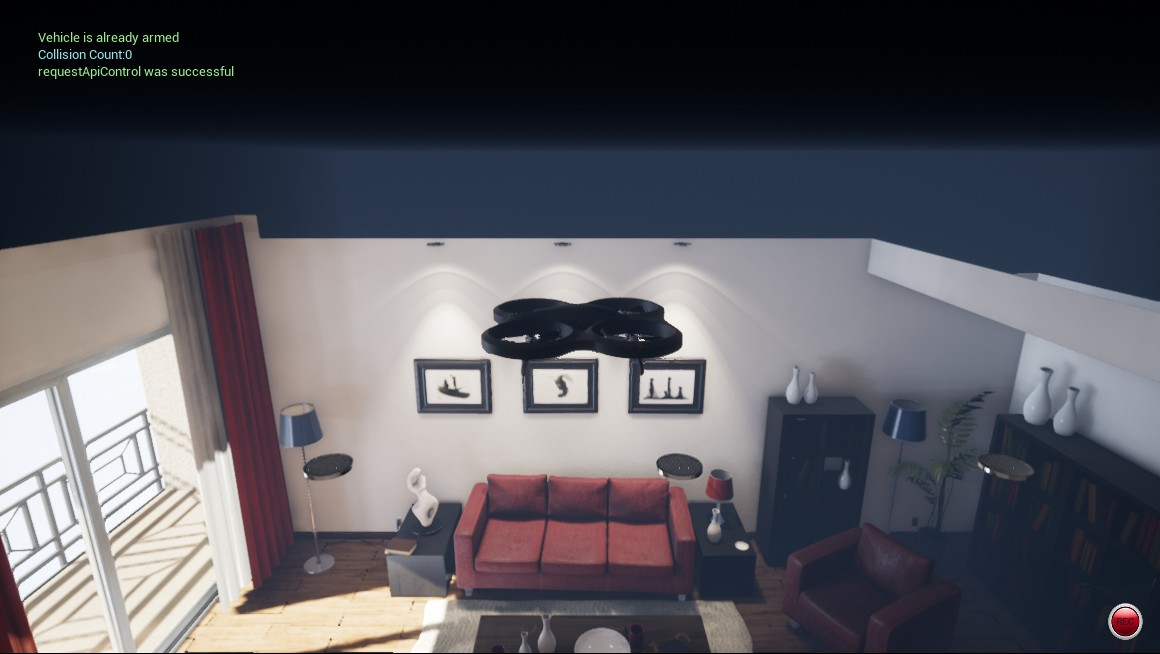
\includegraphics[width = 0.7\textwidth]{rapport/fig/Results/inflight.jpg}
    \caption{Indoor test scene in the Unreal Engine editor}
    \label{fig:res_inflight}
\end{figure}

The simulator will work in any environment created in Unreal Engine, by adding the project specific files along the AirSim files to the new scene. Figure \todo[inline]{add new environment} shows the same simulator in two other environments. The process of using pre-made scenes may be a bit tedious for Linux, since most scenes has been created for Windows. However, Unreal Engine provides tools for converting the projects to support Linux, and as of now all scenes have worked.

\begin{figure}[!htb]
    \centering
    \begin{subfigure}{0.32\textwidth}
    \centering
        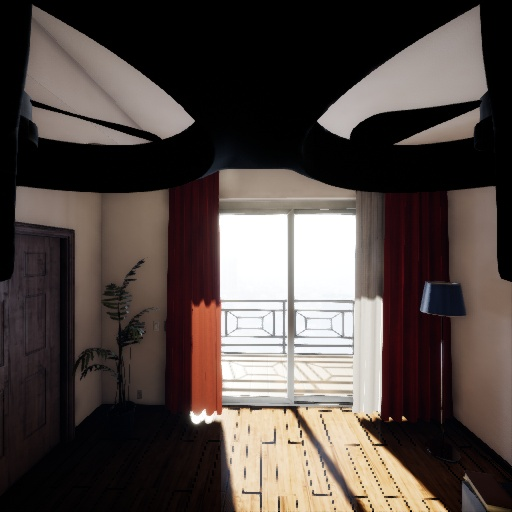
\includegraphics[height=5cm]{rapport/fig/Results/single/forward_center.jpeg}
        \caption{Front Camera}
        \label{fig:res_original_front}
    \end{subfigure}
    \begin{subfigure}{0.32\textwidth}
        \centering
        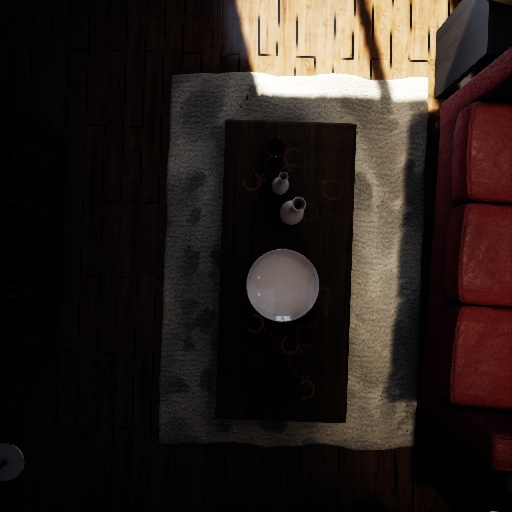
\includegraphics[height=5cm]{rapport/fig/Results/single/down_center.jpeg}
        \caption{Downward camera}
        \label{fig:res_original_down}
    \end{subfigure}    
    \begin{subfigure}{0.32\textwidth}
        \centering
        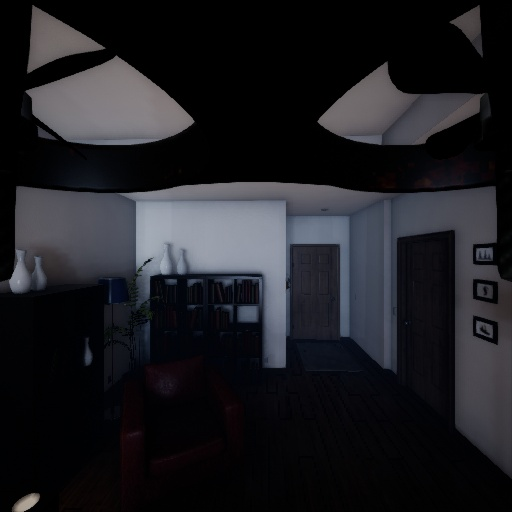
\includegraphics[height=5cm]{rapport/fig/Results/single/backward_center.jpeg}
        \caption{Back camera}
        \label{fig:res_original_back}
    \end{subfigure} \\[0.75ex]
    \begin{subfigure}{0.32\textwidth}
        \centering
        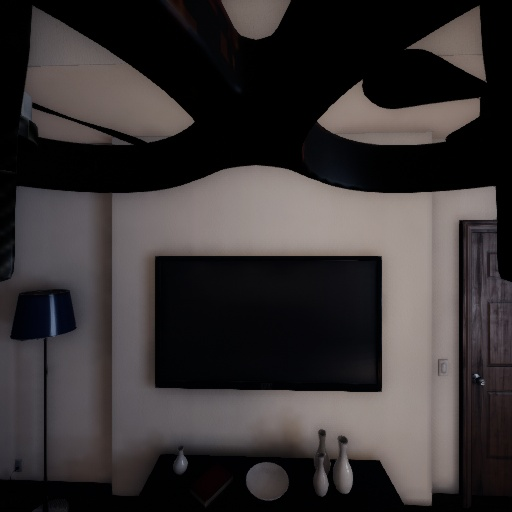
\includegraphics[height=5cm]{rapport/fig/Results/single/left_center.jpeg}
        \caption{Left Camera}
        \label{fig:res_original_left}
    \end{subfigure}
    \begin{subfigure}{0.32\textwidth}
        \centering
        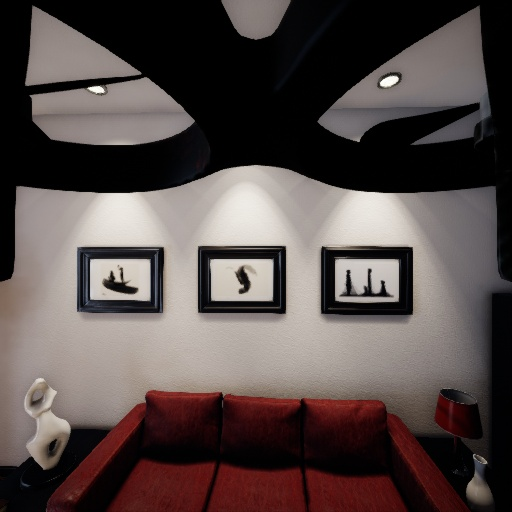
\includegraphics[height=5cm]{rapport/fig/Results/single/right_center.jpeg}
        \caption{Right Camera}
        \label{fig:res_original_right}
    \end{subfigure}
    \centering
    \caption{The original perspective images from Airsim, taken in flight}
    \label{fig:res_original_pictures}
\end{figure}

\subsection{Cube capture and omnidirectional fisheye iamge tranformation}

The perspective images seen in ~\ref{fig:res_original_pictures} were taken were taken from the air, as shown in Figure~\ref{fig:res_inflight}. Since these cameras cover a $360^\circ$ horizontal FoV and a $270^\circ$ vertical FoV, they also capture parts of the multirotor the camera cluster is attatched to. These features will be apparent in the transformed pictures shown later in the section.

Figure~\ref{fig:res_quality_comparison} shows three images taken with different resolution, and using an equiangular projection. The resolution in the compared pictures matches that of the perspective image resolution. This means that the $512\times512$ pixel image is combined from five $512\times512$ pixel images and so on. One can see that the image in Figure~\ref{fig:res_comp_256_to_256} is substantially lower than that of the image in Figure~\ref{fig:res_comp_1024_1024}. Almost all details on the door and railing are lost, and the reflection seen in the plate at the table is almost none existent. Comparing Figure~\ref{fig:res_comp_512_512} and Figure~\ref{fig:res_comp_1024_1024}, the differences are quite minimal.

\begin{figure}[!htb]
    \centering
    \begin{subfigure}{0.45\textwidth}
    \centering
        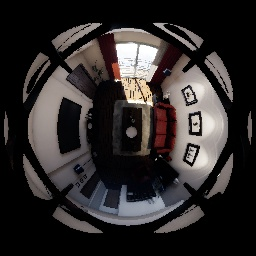
\includegraphics[height=6cm]{rapport/fig/Results/256to256.jpeg}
        \caption{$256 \times 256$ pixels}
        \label{fig:res_comp_256_to_256}
    \end{subfigure}
    \begin{subfigure}{0.45\textwidth}
        \centering
        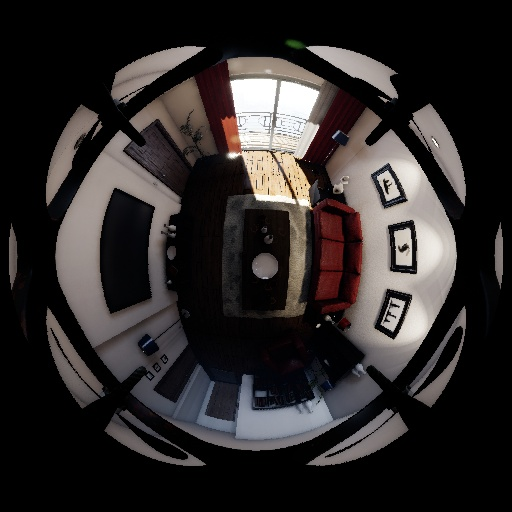
\includegraphics[height=6cm]{rapport/fig/Results/512to512.jpeg}
        \caption{$512 \times 512$ pixels}
        \label{fig:res_comp_512_512}
    \end{subfigure} \\   
    \begin{subfigure}{0.7\textwidth}
        \centering
        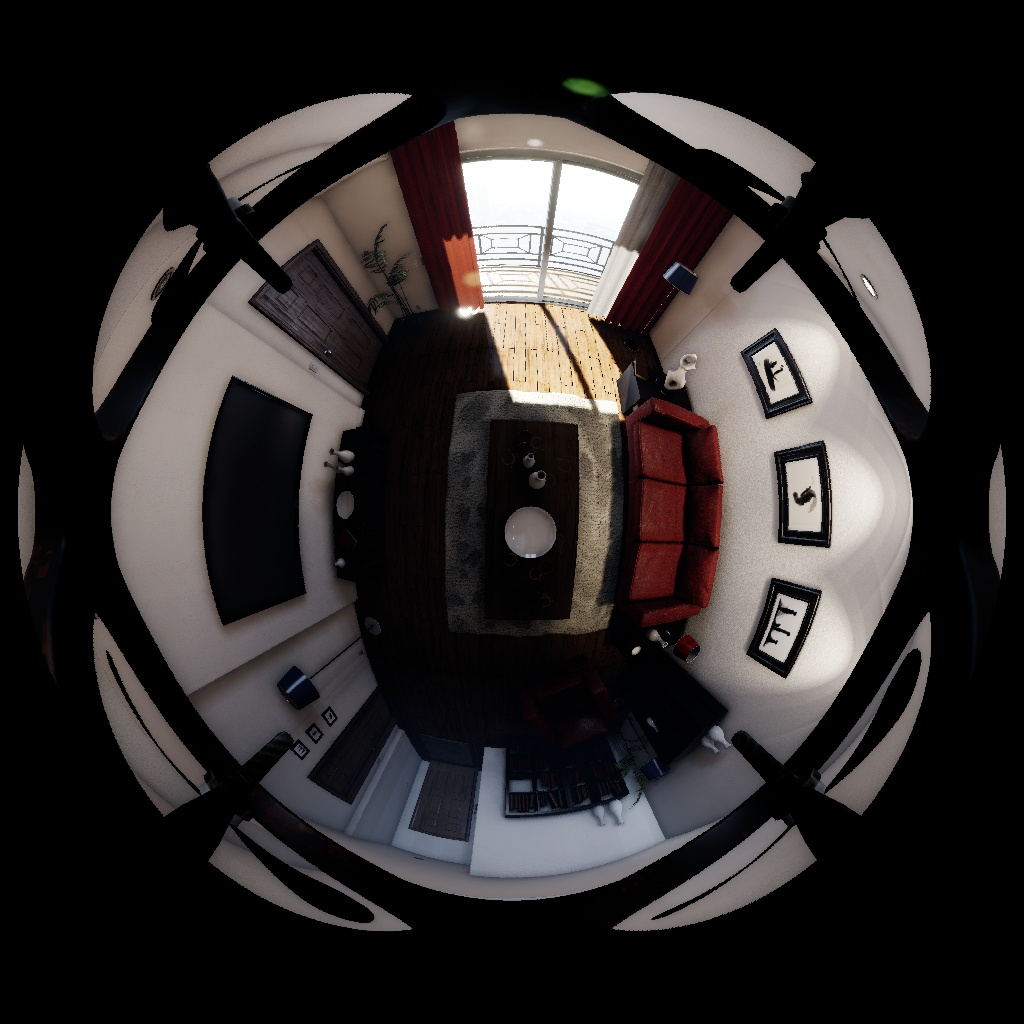
\includegraphics[height=6cm]{rapport/fig/Results/1024to1024.jpeg}
        \caption{$1024 \times 1024$ pixels}
        \label{fig:res_comp_1024_1024}
    \end{subfigure}
    \centering
    \caption{Image quality comparison, where that resolution and of the output picture matches the resolution of the five perspective images}
    \label{fig:res_quality_comparison}
\end{figure}

The images in Figure~\ref{fig:res_comp_equal} are taken with the same perspective image resolution of $512 \times 512$, but with two different destination resolutions. The most important difference here is the distortion lines seen in Figure~\ref{fig:res_comp_equal_512_1024}, caused by the stretching of the source image. However, it can also be seen that the detail level in the central parts have been increased.

\begin{figure}[!htb]
    \centering
    \begin{subfigure}{0.45\textwidth}
        \centering
        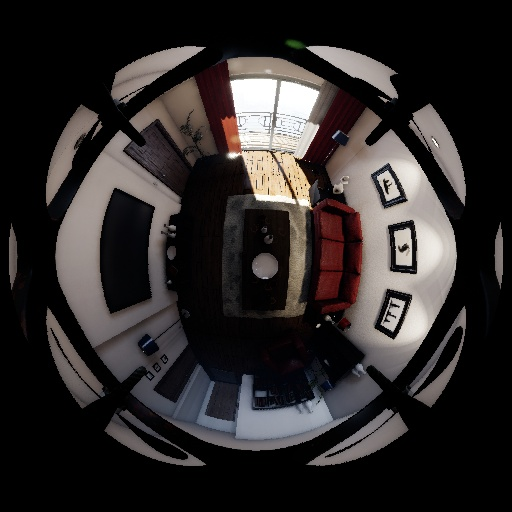
\includegraphics[height=6cm]{rapport/fig/Results/512to512.jpeg}
        \caption{$512 \times 512$ pixels}
        \label{fig:res_comp_equal_512_512}
    \end{subfigure}
    \begin{subfigure}{0.45\textwidth}
        \centering
        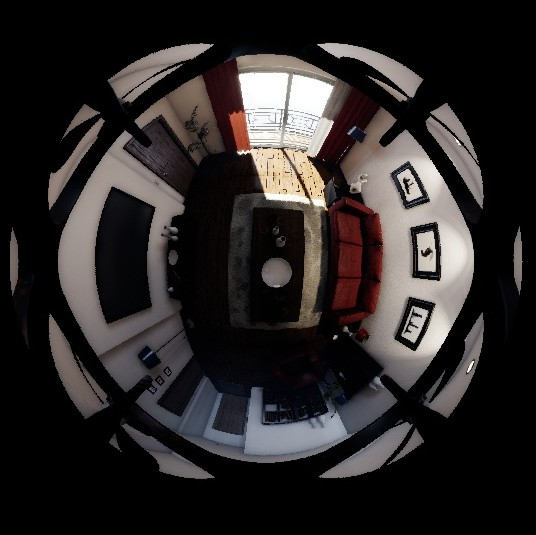
\includegraphics[height=6cm]{rapport/fig/Results/512to1024.jpeg}
        \caption{$1024 \times 1024$ pixels}
        \label{fig:res_comp_equal_512_1024}
    \end{subfigure}
    \caption{Comparison of images transformed from five $512 \times 512$ pixel perspective images}
    \label{fig:res_comp_equal}
\end{figure}

Adding noise and changing exposure settings is integrated into AirSim, and is set in the AirSim settings. Figure~\ref{fig:res_pp} shows three images, where \ref{fig:res_pp_noise_yes} has added noise, both in the form of random pixel intensity and in the form of flickering, noise lines and distortion. The effects have been exagerated to make it visible in the report. All effects can be controlled independently. One thing to note is that these effects are applied to the perspective images. This means that they will be distorted by the fisheye transformer after this effect is applied. This adds extra smudging, especially at higher $\phi$ values. 

\begin{figure}[!htb]
    \centering
    \begin{subfigure}{0.45\textwidth}
        \centering
        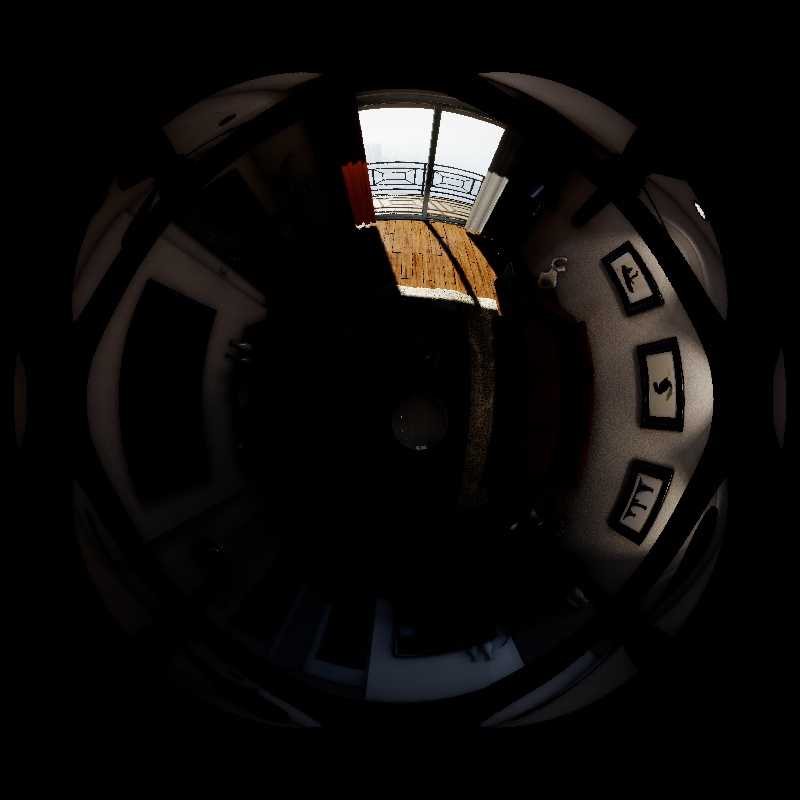
\includegraphics[height=6cm]{rapport/fig/Results/pp/no_nooise_high_min_brightness.jpeg}
        \caption{Low exposure time}
        \label{fig:res_pp_exposure_yes}
    \end{subfigure}
    \begin{subfigure}{0.45\textwidth}
        \centering
        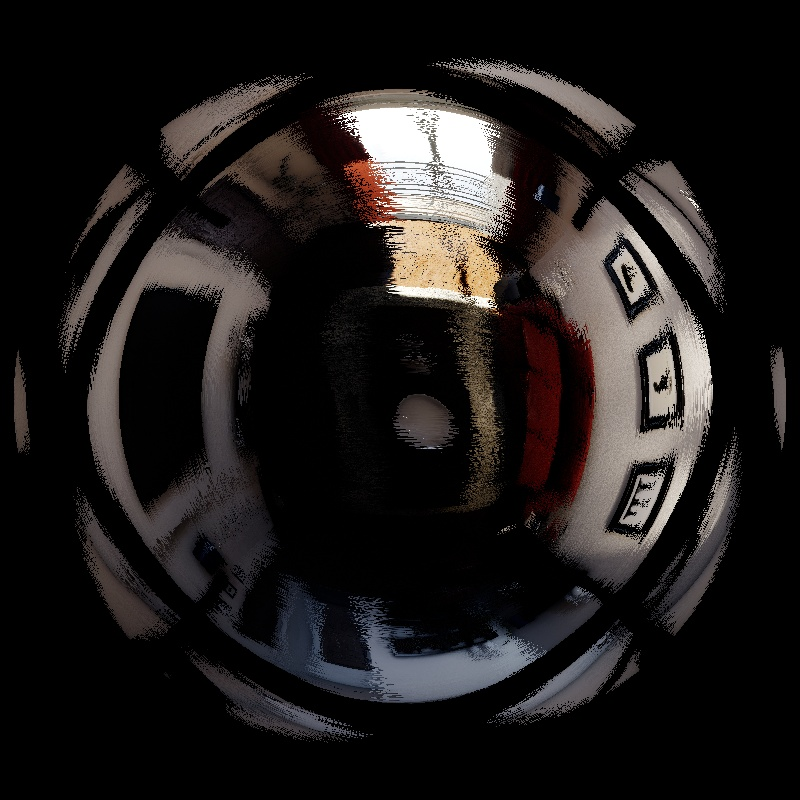
\includegraphics[height=6cm]{rapport/fig/Results/pp/noise_normal_exposure.jpeg}
        \caption{Noisy picture}
        \label{fig:res_pp_noise_yes}
    \end{subfigure}
    \caption{Additional noise and exposure added to the image}
    \label{fig:res_pp}
\end{figure}

Figure~\ref{fig:res_pp_exposure_yes} has had it's exposure massively reduced, and this is also an effect directly integrated by AirSim. The settings allow the user to control the amount of automatic exposure adjustment speed, as well as maximum and minimum values. This effect has been nicely integrated into the fisheye-transformed image, without any apparent side effects. There are manual controls for this in Unreal Engine, but they have not been transferred to AirSim's settings. This is however controlable from the editor directly.

\subsection{Single picture distortion}

Figure~\ref{fig:res_comp_single} shows how single pictures are distorted using the same equidistant lens model. These picture were taken from the front camera on the multirotor, while stationary on the table. The most noticable effect in this picture is the effect the direct sunlight has on the exposure. This makes the rest of the scene appear much darker, which is a normal effect seen in cameras. At low resolutions there are unfortunately some texture clipping, especially of the plant in Figrue~\ref{fig:res_comp_single_256_200}.

\begin{figure}[!htb]
    \centering
    \begin{subfigure}{0.45\textwidth}
        \centering
        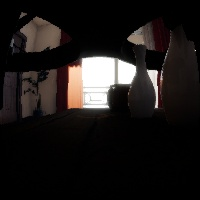
\includegraphics[height=6cm]{rapport/fig/Results/single/single_256_200.jpeg}
        \caption{$200 \times 200$ pixels}
        \label{fig:res_comp_single_256_200}
    \end{subfigure}
    \begin{subfigure}{0.45\textwidth}
        \centering
        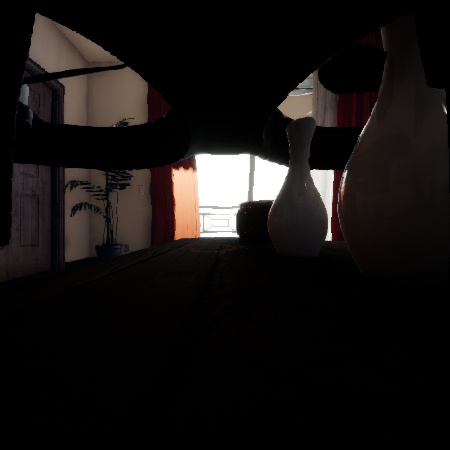
\includegraphics[height=6cm]{rapport/fig/Results/single/single_512_450.jpeg}
        \caption{$450 \times 450$ pixels}
        \label{fig:res_comp_single_512_450}
    \end{subfigure} \\

    \begin{subfigure}{0.45\textwidth}
        \centering
        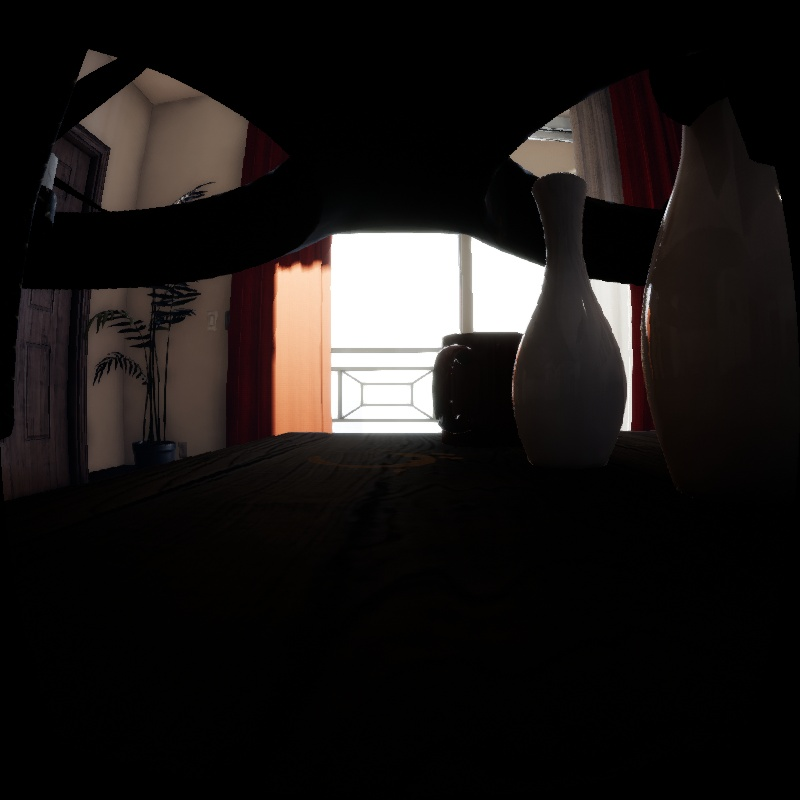
\includegraphics[height=6cm]{rapport/fig/Results/single/single_1024_800.jpeg}
        \caption{$800 \times 800$ pixels}
        \label{fig:res_comp_single_1024_800}
    \end{subfigure}
    \begin{subfigure}{0.45\textwidth}
        \centering
        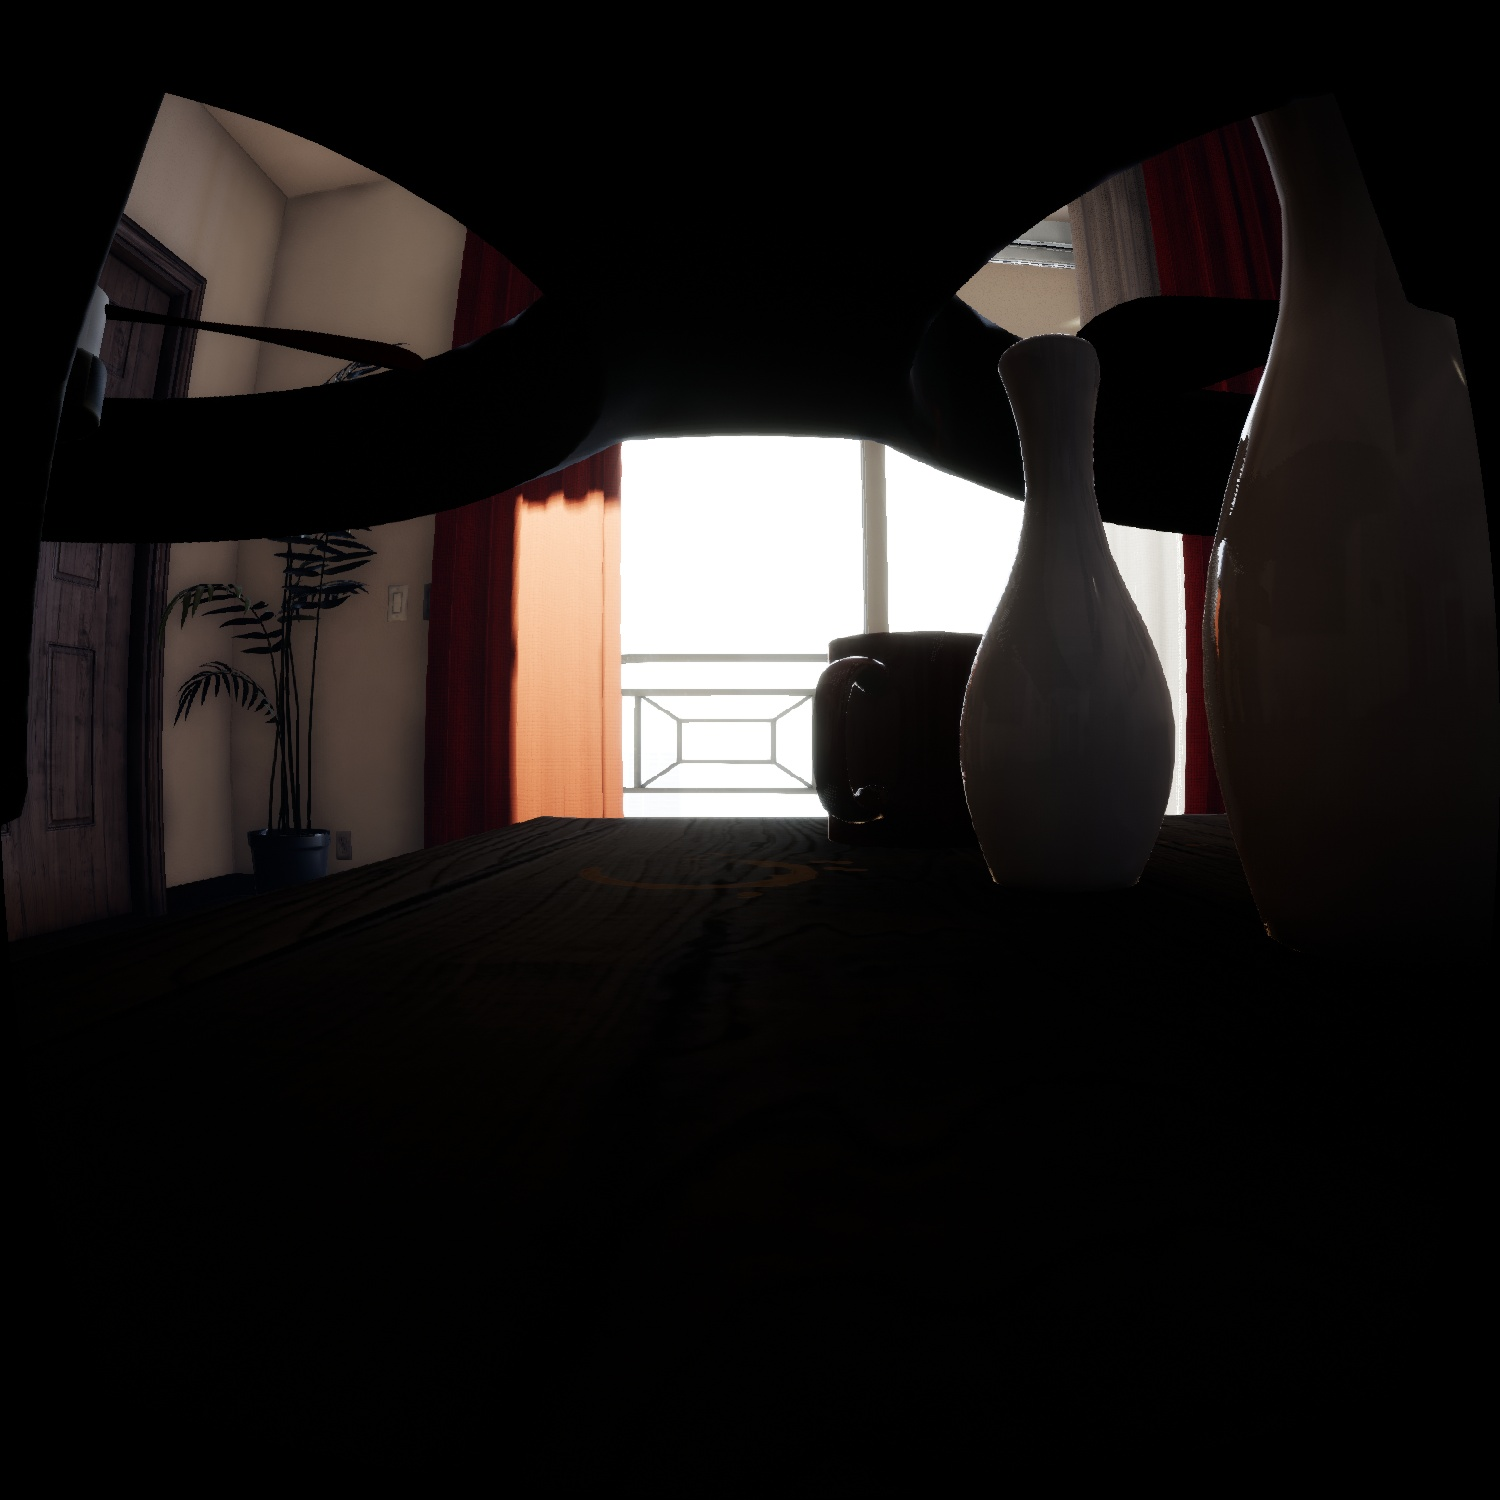
\includegraphics[height=6cm]{rapport/fig/Results//single/single_2048_1500.jpeg}
        \caption{$1500 \times 1500$ pixels}
        \label{fig:res_comp_single_2048_1500}
    \end{subfigure}
    \caption{Transformed images taken based on a single perspective image at different resolutions}
    \label{fig:res_comp_single}    
\end{figure}

The simulator also allows altering of the distortion model. This can be seen in Figure~\ref{fig:res_different_distortions}, where three distortion models are presented. Note that the images are scaled to match the output resolution, as described towards the end of Section~\ref{sec:lens_modeling}. This means that it is the ratio between the parameters which are important, not the actual size. While Figure~\ref{fig:res_different_distortion_k1} shows the equidistant distortion, the two other images show added nonlinear radial distortion. Looking at the vases on the table, this can clearly be seen in Figure~ \ref{fig:res_different_distortion_k1k2k3}. In these picture it is also noticably less radial distortion towards the egdes of the picture, compared to Figure~\ref{fig:res_different_distortion_k1}.

\begin{figure}[!htb]
    \centering
    \begin{subfigure}{0.45\textwidth}
        \centering
        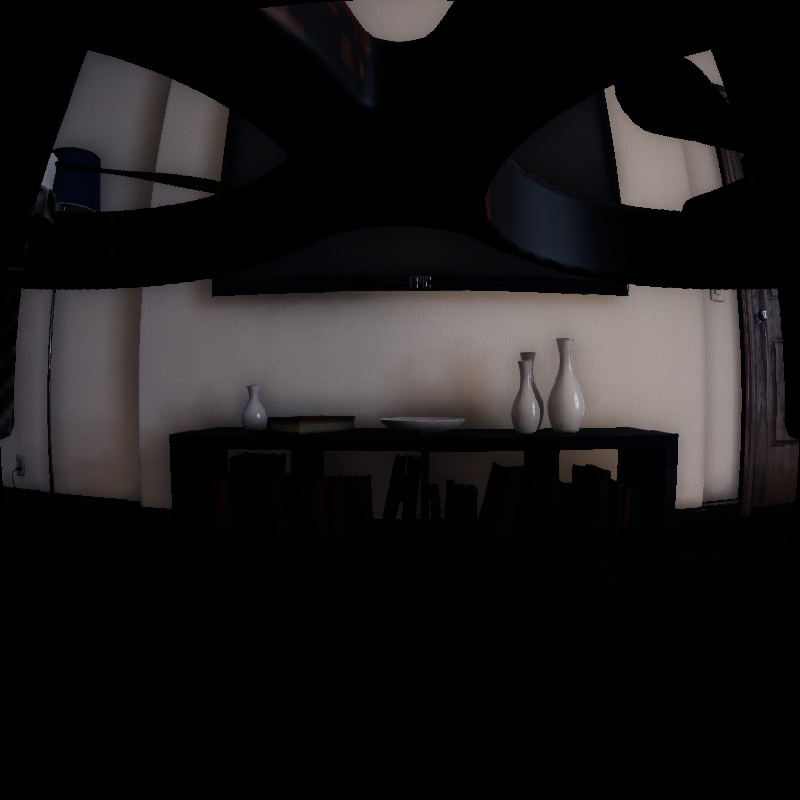
\includegraphics[height=6cm]{rapport/fig/Results/single/single_equi_distort_noline.jpeg}
        \caption{$r(\phi) = 1.0 \cdot \phi$}
        \label{fig:res_different_distortion_k1}
    \end{subfigure}
    \begin{subfigure}{0.45\textwidth}
        \centering
        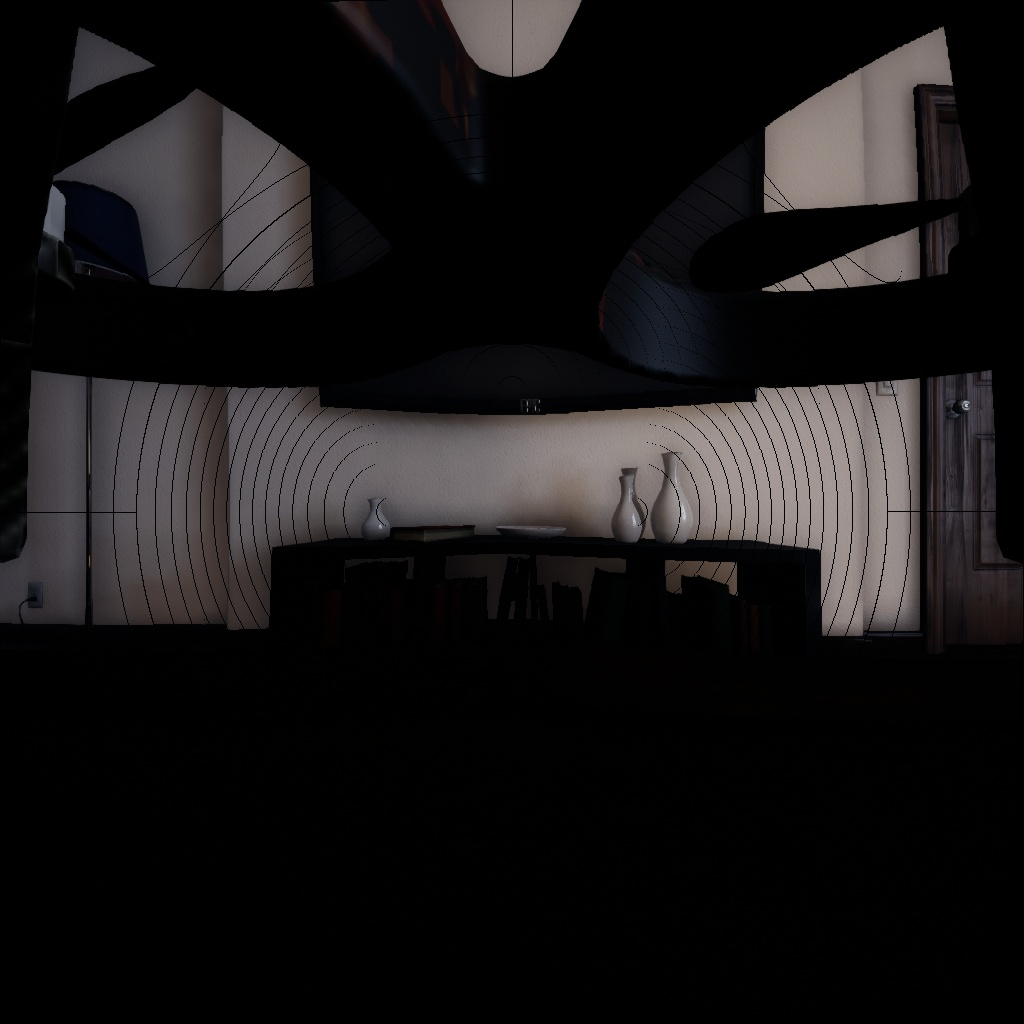
\includegraphics[height=6cm]{rapport/fig/Results/single/single_k2_distort.jpeg}
        \caption{$r(\phi) = 1.0 \cdot \phi + 0.7 \cdot \phi^2 + 0.3 \cdot \phi^3$}
        \label{fig:res_different_distortion_k1k2k3}
    \end{subfigure}
    \caption{Single pictures taken from the frontal camera using different distortion models}
    \label{fig:res_different_distortions}
\end{figure}

Figure~\ref{fig:res_different_distortion_k1k2k3} also shows significant distortion lines in the pictures. As with Figure~\ref{fig:res_comp_equal_512_1024}, this is caused by having too high resolution on the output image compared to the input image. However, for this example it shows the principle of nonlinear radial distortion, where the contour lines have increased spacing, with increasing $\phi$.

\subsection{Performance}

While the performance never was a part of the equation when implementing it, it is an important factor in a control application. All tests have been performed on the office PC in at NTNU. This PC does not have a dedicated graphics card, and Unreal Engine lagged considerably during tests. How much this affected the tests is unknown. however they should show qualitative data to shed some light upon areas to imporve the simulator.

Table~\ref{tab:res_timing_single} and \ref{tab:res_timing_cube_capture} show the timings in seconds for different resolutions and capture types. Note that while this is not even close to real time, all calculations done by the simulator are done sequentially for each pixel in the picture, meaning that no parallellization has been done. This can clearly be seen by comparing the calculation times, where the computation time follows the increase in resolution linearly. The fetch times are also higher for higher resolution picture, which are to be expected. Around $512\times 512$ it became quite noticable. 

\begin{table}[!htb]
    \centering
    \begin{tabular}{|c|c|c|c|} \hline
        \textbf{Input resolution} & \textbf{output resolution} & \textbf{Timing type} & \textbf{Time elapsed} \\ \hline \hline
        \multirow{2}{*}{$256 \times 256$} & \multirow{2}{*}{$512 \times 512$} & Fetch & 0.1 - 0.2 s \\ \cline{3-4}
         & & Transform & 0.4 s \\ \hline
        \multirow{2}{*}{$512 \times 512$} & \multirow{2}{*}{$512 \times 512$} & Fetch & 0.1 - 0.2 s\\ \cline{3-4}
         & & Transform & 1.5 s \\ \cline{2-4}
        \multirow{2}{*}{$1024 \times 1024$} & \multirow{2}{*}{$1024 \times 1024$} & Fetch &  0.3 - 0.5 s \\ \cline{3-4}
         & & Transform & 6.0 s \\ \hline
        \multirow{2}{*}{$2048 \time 2048$} & \multirow{2}{*}{$2048 \times 2048$} & Fetch & 0.6 - 0.7 s\\ \cline{3-4}
         & & Transform & 24.1 s\\ \hline
    \end{tabular}
    \caption{Timing for single capture transformation to fisheye image}
    \label{tab:res_timing_single}
\end{table}

\begin{table}[!htb]
    \centering
    \begin{tabular}{|c|c|c|c|} \hline
        \textbf{Input resolution} & \textbf{output resolution} & \textbf{Timing type} & \textbf{Time elapsed} \\ \hline \hline
        \multirow{2}{*}{$256 \times 256$} & \multirow{2}{*}{$256 \times 256$} & Fetch & 0.3 - 0.4 s\\ \cline{3-4}
         & & Transform & 2.0 s\\ \hline
        \multirow{4}{*}{$512 \times 512$} & \multirow{2}{*}{$512 \times 512$} & Fetch & 0.4 - 0.5 s \\ \cline{3-4}
         & & Transform & 7.9 s\\ \cline{2-4}
         & \multirow{2}{*}{$1024 \times 1024$} & Fetch & 0.4 - 0.5 s\\ \cline{3-4}
         & & Transform & 7.9 s\\ \hline
        \multirow{2}{*}{$1024 \time 1024$} & \multirow{2}{*}{$1024 \times 1024$} & Fetch & 0.7 s\\ \cline{3-4}
         & & Transform & 30.9 s\\ \hline
    \end{tabular}
    \caption{Timing for cube capture transformation to fisheye image}
    \label{tab:res_timing_cube_capture}
\end{table}


\section{Discussion}

While both the $360^\circ$ image capture simulator and the ROS publisher node has been implemented, and is working for their intended purposes, there are still a lot of quirks that needs to be sorted out for this to be a releasable product. The main issue is the performance, in the form of time delay, where a control application running on this simulator needs to get the video feed at a reliable rate in order for the simulator to appear as though it was a real system. Another is usability and available customization, where the simulator should provide the option to add this camera type to different vehicles, different configurations for the multirotor.

On the other hand, the simulator provides great image qualities with lighting effects that are hard to create in other simulators. Effects like the occlusion created on other objects when the camera is exposed to direct sunlight are effects that CV-algorithms have to deal with, but there are limited resources for simulating accurately. Using this simulator, new data sets can be made by recreating environments or just flying along new paths. This is especially powerful for deep learning application, where over-fitting to a small sample size is a common problem. This chapter will discuss these topics in more detail, reflect upon the choises made underways, and present further work and advancement opportunities for the simulator. 

\subsection{Image Quality and captured effects}

While image quality and level of detail in the picture is important, it does often have to be disregarded in control applications due to the time it takes to extract information from large images. Even though this is to some extent less relevant for large moving vehicles like cars and ships, where one can store hardware capable of high amounts computation power, it is highly relevant for smaller objects like the multirotor in this simulator or other small vehicles. However, this does not mean that advanced shader effects, such as reflections are removed. Rather these effects tend to blend into the object coloring, creating even more difficulties for the CV application. This effect can clearly be seen in Figure~\ref{fig:res_comp_single_256_200}, where the reflections of the curtain is still apparent in the vases on the table. However the textures are harder to discern from each other, since less of the contrast is captured.

When it comes to the distortion mapping, the fisheye camera does its job well. The total picture is best shown in Figure~\ref{fig:res_show_fisheye}, and here we clearly see that there are no mismatching textures, or lines resembling the stitching of the images. This would probably have been most apparent in the balcony door, where there is a stitching between the front and downwards pointing camera. It also produces the expected radially increasing distortion effect, and ends up as a circular image on the image plane, as it would with a real fisheye camera. Looking at the original pictures in Figure~\ref{fig:res_original_pictures}, it can be seen that all light and shadow effects have been correctly mapped into the new image, as these effects are also prone to the lens distortion. 

There are problems with the textures on low reasolution pictures, as seen in Figure~\ref{fig:res_comp_256_to_256} where the edges become discrete looking. However, I believe this would also happen with real fisheye cameras that have this low resolution. This is not certain, as I cannot show any results to back up this claim. These problems do however become insignificant at resolutions around $500\times 500$ pixels. Though, as stated by \cite{Zhang2016BenefitOL} the angular resolution of the omnidirectional cameras are a real problem, meaning that resolutions most likely will have to be of this size or higher in any real control application. Especially in outdoor environments.

Another problem seen in the simulator comes when increasing the resolution of the output picture beyond the resolution of each individual pespecive picture. Since the images towards the end of edges of the picture gets stretched much more than the center parts, there are not enough pixels in the original image to map to these points. The effects are seen in Figure~\ref{fig:res_comp_equal_512_1024} and \ref{fig:res_different_distortion_k1k2k3}, where it looks like distortion lines are appearing. This effect would not appear in a real camera, as there would be a continous field of light hitting the whole lens. 

One solution to this may be capturing the horizontal perspective images with a higher resolution than the downward looking camera. Another solution would be to add gradient effects, mapping the outlier pixels with an average of the color of the pixels around it. It is also possible that this problem is completely removed if the scaling with $x_{max}$ and $y_{max}$ shown in Equation~\eqref{eq:impl_pixel_transform_final} is removed, though this has not been tested. 

The scaling is introduces as a way to ensure that the final picture fits the output resolution of the image. This provided an easy way to test the simulator. However it should not be active when calibrating the simulators camera to an actual fisheye camera, as it negates parts of the lens parameters physical relation. As an example, in the equidistant model $r=k_1 \phi$, the $k_1$ parameter directly ties to the focal length of the fisheye camera, mapping the fisheye projection to an image plane with a specific size. In that camera, the photosensitive CCD would also have physical dimentions which may or may not match the image plane. The scaling parameter from Equation~\eqref{eq:impl_pixel_transform_final} would ensure that these match, and therefore give incorrect results.

As the lens model is now, it only incorporates radial distortion in the images. In a real camera one may encounter off center distortions, image stretching due to misalignment of the lens and image plane, tangential distortion or any combinations of these. While the simulator does not incorporate them at this moment, the lens model is made to be changed easily, as it only implements its parameters and a simple distort function, calculating the radius from center for the new pixel. This function can easily be changed in later iteration.

Referring to Section~\ref{sec:Chooseplatform} there was presented a lot of effects that Unreal Engine could produce, that would be much harder, if not impossible to implement into Gazebo. These were shown in the Tables~\ref{tab:comparison_camera} and \ref{tab:comparison_shader}. While few of these effects have been tested agains actual real world footage, many of them are already incorporated naturally in the images shown in the results section. Noise and exposure setting have been tested quite a bit, with two pictures displaying these effects are shown in Figure~\ref{fig:res_pp}.

The exposure settings are controllable through the AirSim settings. Sadly it does not include the manual override of the automatic eye adaption mechanic of Unreal Engine. However, minimum, maximum exposure as well as adaptation speed can be controlled freely. This means that the simulator does not support setting a specific exposure time or shutter speed directly. Most likely the camera which is to be calibrated will have its own automatic exposure settings, and the simulator should be able to match these. It is stated by the developers of AirSim that motion blur is implemented. However, it has not been functioning in any of my attempts. Further investigation is needed, as there may be other post processing elements overwriting this setting.

When it comes to noise in the picture, the simulator unfortunately does not work optimally. While the effects are shown, they are applied to the original perspective images, before they are transformed. This means that especially wave distortion will appear to be stretched out in the image, as seen in Figure~\ref{fig:res_pp_noise_yes}. Reduced noise effects can still be applied with reasonable functionality, but the settings has to be fine tuned, and may suddenly produce unintentional artifacts, especially with random nouise settings applied.

Vignette, is a lens property that is not supported. As the effect encircles the perspective picture, it appears as rings on the transformed image. If this setting is to be supported, it would have to be added as another post processing step in the fisheye transformer. As This is an effect that increases with radius, it could be implemented by scaling the light intesity down, with an increasing radius.

The shader effects shown in Table~\ref{tab:comparison_shader}, are in many cases integrated into the images shown in the results. Looking closely at Figure~\ref{fig:res_show_fisheye}, we see shadows being cast from the picture frames and the sofa, caused by the spot lights on the wall. We also see the that the railings, curtains and door frame cast realisticly looking shadows, based on the outdoor lighting. One special thing to note here is that the table on the door side of the sofa does not cast a shadow. This shown the power of the dynamic shading done by Unreal Engine, as the shadow cast by the spot light is correctly removed by the stronger sunlight. The picture also shows sign of lens flares in the picture in the door area, which is a typical image effect appearing in pictures capturing strong sunlight.

\todo[inline]{finish for table 3.3. Go sleep now}

\subsection{Performance and optimization}

\subsection{Task}

This project has not been a typical cybernetics project, and in many ways it shares more similarities with a computer science project. While the goal of was to extend the project to incorporate calibrating the fisheye camera to an actual camera, and possiby test computer vision algorithms on the platform, there hasn't been time. This is mainly because of lack of experience in critical areas. 

The project has had to handle very large code bases. Both the codebase of Unreal Engine and AirSim is quite extensive, as they both provide lots of functionality and features. While both platforms have a large user base, few of these discuss problems around the source code and the communication patterns within. Information regarding this is mostly limited to Github issues, and a few forum posts. While these problems became less relevant when making the client side application, it was a huge part of the development described in Section~\ref{sec:Early_dev}. 

Since the fisheye model was to be included into the AirSim interface, a deep understanding of the AirSim package was needed. Both in terms of internal dependencies, class and type definitions, coding style and communication patterns. The fact that it also had to incorporate new funtionality fom Unreal Engine meant that knowledge of C++ scripting towards Unreal Engine was needed. As the platform has an enormous amount of tools and funtionality available, there are also a lot of abstractions, to make the interface possible to use and develop for. However, the lack of previous experiece with game engines or Unreal Engine in particular, made this process quite time consuming. While reading through guides and watching tutorials

\subsection{Platform}

% This decision was made in order to separate the implementation into its own module, and thereby reducing the impact of changes to AirSim. As AirSim is still developed heavilly upon, it was seen as a way to reduce the amount trouble induced by changes to the core code of the plugin. This would also allow me to more often integrate the bug fixes and new implementations they made, without ruining my ownw work. The downside of this decision is that it removes possibility to use any features in Unreal Engine which is not implemented in the AirSim API. 


% \subsection{Project setup and programming environment}

% In this project I have forked both the EpicGames/Unreal Engine and the Microsoft/AirSim repository to my Github account, and made my own pivate repository for the project. This enable me to do specific changes to the source code of these projects, without the need to make pull requests to their original repositories. While AirSim is openly available, the source code of Unreal Engine is only available after being registered as a developer through their website. One requirement for getting the source code is that it is not distributed outside of this licencing. For this reason neither the fork of Unreal Engine, nor my own project repository are publicly available.

% Since one of the main goals of this project is the interfacing to ROS, the main OS for development will be Linux, specifically Ubuntu 18.04. However, since Unreal Engine is deeply integrated with Visual Studios, I will use Visual Studios on Windows as the main debugging platform, for everything except ROS. To build on Linux, I will use CMake, as they have done with AirSim. Both Unreal Engine and AirSim is built with the clang compiler, using libc++ as the standard library. However, the default ROS install uses libstdc++ as their standard library. This caused linking problems when combining ROS and AirSim. I therefore had to make some changes to the build and CMake scripts of AirSim in order to build with the GNU compiler g++, using libstdc++ as the standard library.

% \todo[inline]{Do I need to describe why this change is important?}

\cleardoublepage